%\documentclass[10pt, twoside, openright]{report}
\documentclass[10pt, twoside, openany]{report}
\usepackage[paperwidth=5.5in, paperheight=8.5in,
  left=1.5cm, right=1.5cm, top=6mm, bottom=6mm,
  bindingoffset=0.5cm,
  includehead, includefoot,
  headheight=23pt, headsep=6pt, footskip=24pt]{geometry}
\usepackage[utf8]{inputenc}
\usepackage[T1]{fontenc}
\usepackage{helvet} % Helvetica for a classic technical feel
\renewcommand{\familydefault}{\sfdefault}

% Colors based on your box art
\usepackage{xcolor}
\definecolor{boxblack}{cmyk}{0.6,0.4,0.4,1} % Rich black (C60 M40 Y40 K100)
\definecolor{cranered}{cmyk}{0,1,1,0.28} % Origami Red (converted from #B80000)
\definecolor{lightgrey}{cmyk}{0,0,0,0.12} % Light grey (converted from #E0E0E0)
\definecolor{warninggrey}{cmyk}{0,0,0,0.06} % Warning grey (converted from #F0F0F0)

% Graphics and Formatting
\usepackage{graphicx}
% SVGs are converted to PDFs by Makefile using Inkscape
\usepackage{titlesec}
\usepackage{fancyhdr}
\usepackage{array}    % Column formatting (e.g. >{\centering})
\usepackage{booktabs} % Professional tables
\usepackage{longtable}
\usepackage{pagecolor} % For the black cover
\usepackage{caption}
\usepackage{float}
\usepackage{framed}
\usepackage{enumitem}
\usepackage[colorlinks=false, pdfborder={0 0 0}]{hyperref}
\setlist[itemize]{itemsep=3pt, parsep=0pt, topsep=4pt}
\setlist[enumerate]{itemsep=2pt, parsep=0pt, topsep=4pt}

% No paragraph indentation
\setlength{\parindent}{0pt}
\setlength{\parskip}{0.5em}

% Warning and Caution box styles
\newenvironment{warningbox}{%
  \def\FrameCommand{\fboxsep=3mm \fboxrule=1pt \fcolorbox{black}{warninggrey}}%
  \MakeFramed{\advance\hsize-\width \FrameRestore}}%
{\endMakeFramed}

\newenvironment{cautionbox}{%
  \begin{quote}\itshape\textbf{Caution:} }%
{\end{quote}}

% Header/Footer Configuration
\pagestyle{fancy}
\fancyhf{}
\fancyhead[LE,RO]{\textbf{A4092 User's Guide}}
\fancyhead[RE,LO]{\nouppercase{\leftmark}}
\fancyfoot[C]{\thepage}
\renewcommand{\headrulewidth}{0.4pt}

% Section styling
\titleformat{\chapter}[hang]{\Huge\bfseries\color{cranered}}{}{0pt}{}
\titlespacing*{\chapter}{0pt}{-28pt}{20pt}
\titleformat{\section}{\Large\bfseries}{}{0pt}{}
\titleformat{\subsection}{\large\bfseries}{}{0pt}{}

\begin{document}

% =============================================================================
% COVER PAGE (Black with Red Cranes)
% =============================================================================
\begin{titlepage}
    \newpagecolor{boxblack}
    \color{white}
    \thispagestyle{empty}

    \begin{center}
        \vspace*{1cm}
        
\includegraphics[width=0.6\textwidth]{cranes.pdf}

        \vspace{1cm}

        {\fontsize{60}{70}\selectfont \textbf{\textcolor{cranered}{A4092}}} \\
        \vspace{0.5cm}
        {\Huge \textbf{Zorro III SCSI-2}} \\
        \vspace{0.2cm}
        {\LARGE Host Adapter}

        \vfill

        \rule{0.8\textwidth}{0.5pt} \\
        \vspace{0.5cm}
        {\small HIGH PERFORMANCE STORAGE SOLUTION FOR AMIGA COMPUTERS}
        \vspace{1cm}
    \end{center}
\end{titlepage}

% =============================================================================
% FRONT MATTER (White background returns)
% =============================================================================
\nopagecolor
\color{black}

% Blank page
\newpage
\thispagestyle{empty}
\mbox{}

% Reset page counter so cover pages don't count
\setcounter{page}{0}

% Warning page
\newpage
\thispagestyle{empty}
\vspace*{2cm}
\begin{warningbox}
\begin{center}
{\Huge \textbf{WARNING}}
\end{center}

\vspace{0.5cm}

Installation information in this document is for reference only. All installation of internal optional devices or equipment including third-party optional devices or equipment, should be performed by an experienced and knowledgeable technician. All servicing or upgrading of original or optional devices or equipment should also be performed by an experienced and knowledgeable technician.

\vspace{0.5cm}

\textbf{UNAUTHORIZED INSTALLATION, SERVICING OR UPGRADING MAY VOID YOUR WARRANTIES.}
\end{warningbox}

\vspace{2cm}

\noindent This manual provides a general description of various product configurations and features currently planned for inclusion in the product line. The configurations and features described may not be available or otherwise apply to your particular system.

% Copyright page
\newpage
\thispagestyle{empty}

\small
\noindent Copyright \copyright\ 2026 by Stefan Reinauer. This document is licensed under the Creative Commons Attribution-ShareAlike 4.0 International License (CC BY-SA 4.0). You may copy, distribute, and modify this work, provided you give appropriate credit and distribute any modified versions under the same license. See: \url{https://creativecommons.org/licenses/by-sa/4.0/}

\vspace{0.3cm}

\noindent With this document no warranties or representations, either expressed, or implied, are made with respect to the products described herein. The information presented herein is being supplied on an ``AS IS'' basis and is expressly subject to change without notice.

\vspace{0.3cm}

\noindent Amiga is a trademark of Amiga Corporation. Original text based on Commodore Part No 371167-01.

\vspace{0.3cm}

\noindent \textbf{NOTE:} The A4092 is a community-developed open source hardware project and has not been independently tested for regulatory compliance (FCC, CE, etc.). The original Commodore A4091, on which this design is based, was certified to comply with FCC Class B limits. As with any electronic device, this equipment may generate radio frequency energy. If interference to radio or television reception occurs, standard mitigation techniques such as repositioning the receiving antenna, increasing separation from the equipment, or using shielded cables may help.

\normalsize

\tableofcontents

% =============================================================================
% CHAPTER 1: A4092 SCSI HOST ADAPTER
% =============================================================================
\chapter{A4092 SCSI Host Adapter}
\label{ch:a4092-scsi-host-adapter}

The A4092 SCSI host adapter is a high-performance board that connects up to seven SCSI devices to your Amiga. The board installs in a Zorro III expansion slot and contains the following features:

\begin{itemize}
    \item Full Zorro III implementation
    \item SCSI-2 implementation
    \item SCSI internal connector and ribbon cable
    \item High density SCSI-2 external connector
    \item Direct Memory Access (DMA) for fast transfers
\end{itemize}

This guide tells you how to:

\begin{itemize}
    \item Check for Zorro III compatibility
    \item Install the A4092 board in an Amiga
    \item Configure SCSI addresses and termination
    \item Install internal and external SCSI devices
    \item Configure a hard drive
\end{itemize}

\newpage

% =============================================================================
% ABOUT OPEN SOURCE
% =============================================================================
\section{About Open Source}
\label{sec:about-open-source}

The A4092 is a community-driven project built on the belief that hardware should be accessible, repairable, and improvable by anyone. We believe in the right to repair and for anyone to make their own version. That is why this product, including all hardware and software, is 100\% open source.

All design files, schematics, PCB layouts, firmware, and software are freely available. You are welcome to:

\begin{itemize}
    \item Study how the board works
    \item Build your own A4092 from the published designs
    \item Modify and improve the design for your own needs
    \item Share your improvements with the community
\end{itemize}

For access to the source files and to contribute, visit the project repository at \url{https://github.com/A4091/a4092}.

% =============================================================================
% RELATED DOCUMENTS
% =============================================================================
\section{Related Documents}
\label{sec:related-documents}

Most instructions and illustrations in this guide refer to an Amiga 4000 Desktop system.
Along with this guide, you will need to refer to your system's hardware user
guide and software guides, including the \textit{Workbench User's Guide}. You
should also check the additional documentation on the A4092 Support disk.

% =============================================================================
% BEFORE YOU BEGIN
% =============================================================================
\section{Before You Begin}
\label{sec:before-you-begin}

Select a clean, well-lit work space. Place your system unit on a stable work surface large enough to accommodate the components of the system unit you remove and replace.

As you work with your system you must:

\begin{itemize}
    \item Protect yourself from electrical shock by turning the Amiga off, unplugging, and disconnecting all cables before removing the cover.
    \item Protect your system from electrostatic discharge (ESD).
\end{itemize}

% =============================================================================
% ESD PRECAUTIONS
% =============================================================================
\section{ESD Precautions}
\label{sec:esd-precautions}

Integrated circuit (IC) chips are sensitive to static electricity. When handling electronic components containing IC chips, including expansion boards and RAM modules, always take precautions to reduce the chances of electrostatic discharge (ESD) harming the components.

Touching a nearby grounded metal surface before touching a component drains static electricity, reducing the likelihood of ESD damage.

To protect your system from ESD, observe these precautions:

\begin{itemize}
    \item Do not unpack any computer components that are wrapped in anti-static packing material until you are ready to install them.
    \item Discharge any static buildup as you work by periodically touching an unpainted metal surface, e.g. on a radiator. This is particularly important before you unpack a new computer component.
    \item Handle each component carefully. Avoid touching card edge connectors, electrical component connectors, and contact points.
\end{itemize}

% =============================================================================
% CHECKING FOR ZORRO III COMPATIBILITY
% =============================================================================
\section{Checking for Zorro III Compatibility}
\label{sec:checking-zorro-iii}

To ensure that your Commodore Amiga 3000 or 4000 system is compatible with the
A4092 SCSI Host Adapter board, the Super Buster chip on your system motherboard
must be (at least) revision 11 (part number 390539-11 or later) for stable Zorro III DMA operation.

\begin{warningbox}
\textbf{Warning:} Turn off your system and unplug the Amiga before checking the
revision of the chip. Disconnect cables for all external peripherals.
\end{warningbox}

To determine whether the chip installed in your system is the correct revision:

\begin{enumerate}
    \item Remove the system cover as described in the \textit{A4000 User's Guide} or \textit{Introducing the Amiga 3000} depending on your model.
    \item Carefully remove any expansion boards that obstruct your view of the chip, shown in Figure~\ref{fig:motherboard}. Refer to the \textit{A4000 User's Guide} or \textit{Introducing the Amiga 3000} for detailed instructions on removing expansion boards from your Amiga model.
    \item The chip can either be socketed or surface-mounted (soldered) on the motherboard. Check the part number on the chip. If the suffix is nine or less, it must be replaced.
    \item Replace the expansion boards.
    \item If your system contains the correct version of the chip and you have already installed the A4092 SCSI host adapter, replace the system cover and reconnect peripheral equipment. If you haven't installed the SCSI host adapter, you can install it now as described in this guide.
    \item Replace the system cover.
\end{enumerate}

\begin{cautionbox}
Some board revisions use a socketed chip that can be replaced directly. Others
require soldering and advanced repair skills. If you are unsure which version
you have, or how to safely upgrade, consult an experienced Amiga hardware technician or a skilled member of the Amiga repair community.
\end{cautionbox}

\begin{figure}[ht]
    \centering
    \includegraphics[width=0.45\textwidth]{figures/figure1-a4000-motherboard.png}
    \caption{Super Buster Location on A4000}
    \label{fig:motherboard}
\end{figure}

% =============================================================================
% CHAPTER 2: INSTALLING THE A4092
% =============================================================================
\chapter{Installing the A4092}
\label{ch:installing-the-a4092}

You can connect up to seven SCSI devices (including hard drives, scanners, tape units and CD-ROMs) to your Amiga using the A4092 board illustrated in Figure~\ref{fig:board}.

\begin{figure}[ht]
    \centering
    \includegraphics[width=0.9\textwidth]{figures/figure2-a4092-board.png}
    \caption{The A4092 SCSI Host Adapter Board}
    \label{fig:board}
\end{figure}

You connect internal SCSI devices to the internal connector with the ribbon cable provided.
In order to connect external SCSI devices, you will have to connect the
A4092 External Connector Bracket to the A4092 using a 50pin SCSI cable.
You connect one external device to the external SCSI connector on the bracket, then connect additional devices in a chain from the first device.

\begin{figure}[ht]
    \centering
    \includegraphics[width=0.9\textwidth]{figures/figure3-external-bracket.png}
    \caption{The A4092 External Connector Bracket}
    \label{fig:bracket}
\end{figure}

\newpage

% =============================================================================
% INSTALLATION STEPS
% =============================================================================
\section{Installation Steps}
\label{sec:installation-steps}

Installing the A4092 board is similar to installing any expansion board in your system. Before you install the board, you should review the configuration options described in ``Configuring the A4092''.

To install the board, do the following:

\begin{enumerate}
    \item Turn off the Amiga's power switch, remove all connecting cables and disconnect the Amiga from the AC power outlet.
    \item Remove the Amiga cover.
    \item Remove the cover plate of the slot in which you intend to install the board. Install the board in any available Zorro III slot.

    \item Look at the 50-pin SCSI ribbon cable, illustrated in Figure~\ref{fig:ribboncable}. Locate the end of the ribbon cable that you will connect to the board. Note that the colored edge of the cable indicates pin 1.

    \item Connect the ribbon cable to the board, aligning pin 1 on the cable connector (colored edge) with pin 1 on the board as illustrated in Figure~\ref{fig:ribbontoboard}.

    \item Insert the board in the slot and attach with the screw from the slot cover plate.

    \item Unplug the hard disk front panel LED cable from the hard disk LED connector on the motherboard (if connected) and plug it into the LEDs header on the A4092 board, illustrated in Figure~\ref{fig:ledheaders}. Use the header labelled A4000 or A3000 depending on your system. On the Amiga 3000, polarity matters---check the triangle marking next to the A3000 LED header in Figure~\ref{fig:ledheaders} to ensure correct orientation.

    \item In order to connect the LED signals from the motherboard, install the LED jumper cable (supplied with the A4092 board) from the motherboard LED connector (CN351 on A4000D, CN302 on A3000D) to the Mainboard header on the A4092 board, illustrated in Figure~\ref{fig:ledheaders}.

\begin{figure}[ht]
    \centering
    \includegraphics[width=0.7\textwidth]{figures/figure4-led-headers.png}
    \caption{LED Header Connections on the A4092}
    \label{fig:ledheaders}
\end{figure}

    \item Install any internal SCSI devices (optional) as described in ``Installing Internal SCSI Devices''.

    \item Replace the Amiga cover.

    \item Install any external SCSI devices (optional) as described in ``Installing External SCSI Devices''.

    \item Reattach connecting cables, reconnect the Amiga to the AC power outlet and turn the power switch on.

    \item The Workbench screen should show a disk icon for each partitioned hard drive you connected. If you installed a new hard drive, see ``Configuring a Hard Drive''.
\end{enumerate}

\begin{figure}[ht]
    \centering
    \includegraphics[width=0.95\textwidth]{figures/figure5-ribbon-cable.png}
    \caption{50-pin SCSI Ribbon Cable}
    \label{fig:ribboncable}
\end{figure}

\begin{figure}[ht]
    \centering
    \includegraphics[width=0.95\textwidth]{figures/figure6-ribbon-to-board.png}
    \caption{Connecting the Ribbon Cable to the Board}
    \label{fig:ribbontoboard}
\end{figure}

\begin{cautionbox}
It is essential to align pin 1 on the cable with pin 1 on your SCSI device. The folds in the provided ribbon cable enable you to easily align pin 1 on the cable with pin 1 on most devices.

Some SCSI devices have reversed the location of pin 1. If you have such a device, you must carefully manipulate the cable to ensure that pin 1 alignment is correct. Failure to align pin 1 can result in damage to the SCSI device.
\end{cautionbox}

% =============================================================================
% CHAPTER 3: CONFIGURING THE A4092
% =============================================================================
\chapter{Configuring the A4092}
\label{ch:configuring-the-a4092}

The A4092 is configured through a boot menu that allows you to control the SCSI address of the board as well as features such as SCSI Fast Bus, short/long spinup, synchronous mode and external termination.

% =============================================================================
% THE BOOTMENU
% =============================================================================
\section{The Bootmenu}
\label{sec:bootmenu}

You can enter the A4092 boot menu by pressing the right mouse button or the DEL key during system startup. The boot menu provides access to all configuration options for the board.

\begin{figure}[ht]
    \centering
    \includegraphics[width=0.8\textwidth]{figures/bootmenu-main.png}
    \caption{A4092 Boot Menu Main Screen}
    \label{fig:bootmenu-main}
\end{figure}

The boot menu contains four main buttons:

\begin{itemize}
    \item \textbf{Disks} --- View and select connected SCSI devices
    \item \textbf{DIP Switches} --- Configure board settings
    \item \textbf{About} --- Display version and credits information
    \item \textbf{Debug} --- Access advanced debugging options
\end{itemize}

Press the \textbf{Boot} button to exit the boot menu and continue the system startup.

% =============================================================================
% DISKS
% =============================================================================
\section{Disks}
\label{sec:disks}

The Disks screen displays all SCSI devices detected on the bus. From here you can view device information and select which device to boot from.

\begin{figure}[ht]
    \centering
    \includegraphics[width=0.8\textwidth]{figures/bootmenu-disks.png}
    \caption{A4092 Boot Menu Disks Screen}
    \label{fig:bootmenu-disks}
\end{figure}

% =============================================================================
% DIP SWITCH
% =============================================================================
\section{DIP Switches}
\label{sec:dip-switches}

Unlike its predecessors, the A4092 does not have physical DIP switches on the board. Instead, all settings are configured through virtual DIP switches in the boot menu. These settings are stored in non-volatile memory and persist across reboots.

\begin{figure}[H]
    \centering
    \includegraphics[width=0.8\textwidth]{figures/bootmenu-dipswitches.png}
    \caption{A4092 Boot Menu DIP Switches Screen}
    \label{fig:bootmenu-dipswitches}
\end{figure}

The virtual DIP switch provides eight switches with two settings each: OFF (open) and ON (closed). The default setting for all eight switches is OFF.

The following table explains the purpose of each switch; note that switches 1, 2 and 3 are used in combination.

\begin{center}
\small
\setlength{\tabcolsep}{4pt}
\begin{longtable}{@{}p{2.0cm}>{\centering\arraybackslash}p{1.0cm}p{2.0cm}p{4.5cm}@{}}
\toprule
\textbf{Switch} & \textbf{Default} & \textbf{Setting} & \textbf{Function} \\ \midrule
\endfirsthead
\toprule
\textbf{Switch} & \textbf{Default} & \textbf{Setting} & \textbf{Function} \\ \midrule
\endhead

\textbf{SCSI \newline Address} \newline 1, 2, 3 & OFF & \raisebox{-0.4\height}{\includegraphics[height=1.2cm,width=2.0cm,keepaspectratio]{figures/dip-switch-address7.pdf}} & Set the SCSI address for the board. See ``SCSI Addresses'' for more information. \\ \addlinespace

\textbf{SCSI \newline Fast Bus} \newline 4 & OFF & \raisebox{-0.4\height}{\includegraphics[height=1.2cm,width=2.0cm,keepaspectratio]{figures/dip-switch-4on.pdf}} & OFF indicates that the SCSI Fast Bus feature is enabled. Set this switch to ON if none of your SCSI devices support SCSI Fast Bus. \\ \addlinespace

\textbf{Short/Long Spinup} \newline 5 & OFF & \raisebox{-0.4\height}{\includegraphics[height=1.2cm,width=2.0cm,keepaspectratio]{figures/dip-switch-5on.pdf}} & OFF indicates that your system uses the standard spinup (booting) time. Set this switch to ON to request a longer booting period. \\ \addlinespace

\textbf{Synchronous Mode} \newline 6 & OFF & \raisebox{-0.4\height}{\includegraphics[height=1.2cm,width=2.0cm,keepaspectratio]{figures/dip-switch-6on.pdf}} & OFF indicates that the synchronous mode feature is enabled. Set this switch to ON to disable synchronous mode. \\ \addlinespace

\textbf{External \newline SCSI \newline Termination} \newline 7 & OFF & \raisebox{-0.4\height}{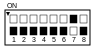
\includegraphics[height=1.2cm,width=2.0cm,keepaspectratio]{figures/dip-switch-7on.pdf}} & OFF indicates that you do not have any external devices. This activates the terminator on the board. Set to ON when you install an external device. \\ \addlinespace

\textbf{Logical Unit (LUN) Enable} \newline 8 & OFF & \raisebox{-0.4\height}{\includegraphics[height=1.2cm,width=2.0cm,keepaspectratio]{figures/dip-switch-8on.pdf}} & OFF indicates that unit 0 is the only unit recognized. Set this switch to ON to enable the system to recognize 1--6 as LUNs. \\
\bottomrule
\end{longtable}
\end{center}

% =============================================================================
% SCSI ADDRESSES
% =============================================================================
\section{SCSI Addresses}
\label{sec:scsi-addresses}

Each SCSI device controlled by the board must have a unique identifier known as the SCSI address. The board must also have a SCSI address. SCSI addresses range from 0 to 7 and must be unique (two devices cannot share an address; a device and the board cannot share an address).

Before you begin installing the board and/or SCSI devices, you must choose the
SCSI address for each device in the SCSI chain. For example, select 7 as the address for the board (the default address set at the factory), 0 and 1 for two internal devices, and 4 for an external device.

Jumpers or switches on a SCSI device determine the SCSI bus identification (SCSI address) for the device. Refer to the device documentation to set the SCSI address for each device.

The first three DIP switches on the board determine the board's SCSI address. If you choose to change the SCSI address from the default, set switches 1, 2 and 3 according to the following table.

\begin{table}[ht]
\centering
\caption{SCSI Address Selection (Switches 1--3)}
\label{tab:scsi_addr}
\begin{tabular}{ccccc}
\toprule
\textbf{SCSI Address} & \textbf{Switch 1} & \textbf{Switch 2} & \textbf{Switch 3} & \textbf{Diagram} \\ \midrule
0 & ON & ON & ON & \raisebox{-0.4\height}{\includegraphics[height=0.8cm]{figures/dip-switch-address0.pdf}} \\
1 & OFF & ON & ON & \raisebox{-0.4\height}{\includegraphics[height=0.8cm]{figures/dip-switch-address1.pdf}} \\
2 & ON & OFF & ON & \raisebox{-0.4\height}{\includegraphics[height=0.8cm]{figures/dip-switch-address2.pdf}} \\
3 & OFF & OFF & ON & \raisebox{-0.4\height}{\includegraphics[height=0.8cm]{figures/dip-switch-address3.pdf}} \\
4 & ON & ON & OFF & \raisebox{-0.4\height}{\includegraphics[height=0.8cm]{figures/dip-switch-address4.pdf}} \\
5 & OFF & ON & OFF & \raisebox{-0.4\height}{\includegraphics[height=0.8cm]{figures/dip-switch-address5.pdf}} \\
6 & ON & OFF & OFF & \raisebox{-0.4\height}{\includegraphics[height=0.8cm]{figures/dip-switch-address6.pdf}} \\
\textbf{7 (default)} & \textbf{OFF} & \textbf{OFF} & \textbf{OFF} & \raisebox{-0.4\height}{\includegraphics[height=0.8cm]{figures/dip-switch-address7.pdf}} \\
\bottomrule
\end{tabular}
\end{table}

% =============================================================================
% SCSI DEVICE TERMINATION
% =============================================================================
\section{SCSI Device Termination}
\label{sec:scsi-device-termination}

A chain of SCSI devices must have two and only two termination points, one at either end of the chain of devices. A terminator indicates the end of the chain (bus) and protects the SCSI devices from potential failure. For the best results with SCSI Fast Bus enabled (switch 4 set to OFF), the terminator at both ends should be active, rather than passive.

For internal devices, an active terminator is attached to the end of the supplied ribbon cable. Before you install an internal device, remove or deactivate the terminator on the device. Refer to the manufacturer's documentation for terminator information.

If you have no external devices, set switch 7 to OFF. This enables the active termination on the board, since this is the other end of the chain.

If you install external devices:

\begin{enumerate}
    \item Verify that switch 7 is set to ON.
    \item Terminate the last SCSI device in the chain. For best results, use active termination. If the device has termination built in, you can enable it, or you can attach an external terminator. If you use passive termination, SCSI Fast Bus should not be enabled (set switch 4 to ON).
    \item Remove or deactivate the terminator from each external device (except for the last one). Refer to the manufacturer's documentation for terminator information.
\end{enumerate}

% =============================================================================
% DEBUG
% =============================================================================
\clearpage
\section{Debug}
\label{sec:debug}

The Debug screen provides access to advanced options that may be useful for troubleshooting or special configurations.

\begin{figure}[ht]
    \centering
    \includegraphics[width=0.8\textwidth]{figures/bootmenu-debug.png}
    \caption{A4092 Boot Menu Debug Screen}
    \label{fig:bootmenu-debug}
\end{figure}

The following options are available:

\begin{itemize}
    \item \textbf{CDROM Boot} --- Enable or disable booting from CD-ROM devices. Disabling this can speed up boot time if you do not have a bootable CD-ROM.

    \item \textbf{Ignore RDBFF\_LAST} --- When enabled, the driver ignores the ``Last Drive'' flag in the Rigid Disk Block (RDB) of SCSI devices. Normally, the system stops scanning for additional partitions when it encounters a partition marked as ``last.'' Enabling this option forces the driver to continue scanning, which can be useful if a disk has incorrectly set partition flags.

    \item \textbf{Quick Interrupts} --- Enable or disable Quick Interrupts for Zorro III DMA transfers. Quick Interrupts can provide faster performance but may cause compatibility issues with some accelerator boards. If you experience system instability, try disabling this option.

    \item \textbf{Allow Disconnect} --- Enable or disable SCSI disconnect/reconnect. When enabled, SCSI devices can disconnect from the bus during long operations and reconnect when ready. Keeping this option disabled helps with certain SCSI devices that do not properly support disconnect/reconnect.
\end{itemize}

% =============================================================================
% ABOUT
% =============================================================================
\section{About}
\label{sec:about}

The About screen displays the firmware version number and provides a small homage to the people who brought you the original A4091 as well as this product.

\begin{figure}[H]
    \centering
    \includegraphics[width=0.8\textwidth]{figures/bootmenu-about.png}
    \caption{A4092 Boot Menu About Screen}
    \label{fig:bootmenu-about}
\end{figure}

% dummy new page to get page count to 36
\newpage
\mbox{}
\newpage

% =============================================================================
% CHAPTER 4: INSTALLING INTERNAL SCSI DEVICES
% =============================================================================
\chapter{Installing Internal \newline SCSI Devices}
\label{ch:installing-internal-scsi}

To install an internal SCSI device in one of the drive bays after the board is installed, follow the steps below.

\begin{enumerate}
    \item Set the address jumper of the device to a SCSI address not used by the board or any other SCSI device.

    \item Remove or deactivate the terminator on the device. See ``SCSI Device Termination'' for more information.

    \item Install the device as described in your hardware user's guide and the device installation manual.

    \item Connect the device to the internal power supply.

    \item Repeat steps 1 through 4 until all internal devices are installed.

    \item If you have installed the board for the first time with the ribbon cable attached:
    \begin{enumerate}
        \item[(a)] Remove the brace on top of the daughterboard by removing the screws that attach the brace to the frame of the Amiga, illustrated in Figure~\ref{fig:brace}.
        \item[(b)] Place the ribbon cable across the notch in the daughterboard.
        \item[(c)] Reattach the brace to the Amiga frame.
    \end{enumerate}

    \item Fold the ribbon cable down and guide it towards the back of the Amiga as illustrated in Figure~\ref{fig:ribbontodevices}.

    \item Connect the ribbon cable to the internal SCSI devices as illustrated in Figure~\ref{fig:ribbontodevices}. Be sure to align pin 1 on the cable connector with pin 1 on the device, usually indicated on the device by an arrow ($\leftarrow$) or the number 1.
\end{enumerate}

\begin{figure}[ht]
    \centering
    \includegraphics[width=0.85\textwidth]{figures/figure7-brace-removal.png}
    \caption{Removing the Brace over the Daughterboard}
    \label{fig:brace}
\end{figure}

\begin{figure}[ht]
    \centering
    \includegraphics[width=0.8\textwidth]{figures/figure8-ribbon-to-devices.png}
    \caption{Connecting the Ribbon Cable to SCSI Devices}
    \label{fig:ribbontodevices}
\end{figure}

\begin{cautionbox}
It is essential to align pin 1 on the cable with pin 1 on your SCSI device. The folds in the provided ribbon cable enable you to easily align pin 1 on the cable with pin 1 on most devices.

Some SCSI devices have reversed the location of pin 1. If you have such a device, you must carefully manipulate the cable to ensure that pin 1 alignment is correct. Failure to align pin 1 can result in damage to the SCSI device.
\end{cautionbox}

% =============================================================================
% CHAPTER 5: INSTALLING EXTERNAL SCSI DEVICES
% =============================================================================
\chapter{Installing External \newline SCSI Devices}
\label{ch:installing-external-scsi}

To connect an external SCSI device after the board is installed in your Amiga, do the following:

\begin{enumerate}
    \item Turn off the power switch and disconnect the Amiga from the AC power outlet.

    \item Verify that switch 7 (External SCSI Termination) on the board is set to ON.

    \item Set the address jumper of the first external SCSI device to an address not used by the board or any internal SCSI device.

    \item Insert the connector of the SCSI device cable (or adapter) into the external SCSI connector on the A4092 External Connector Bracket, illustrated in Figure~\ref{fig:externalconnector}. Align the two pieces to slide straight into one another, since they fit tightly together. Push until the retaining clips are secured. Press the rectangular pieces of metal on either side of the connector to release the retaining clips when inserting or removing the connector.

    \item Set the address jumper of each succeeding SCSI device to an unused SCSI address.

    \item Connect each succeeding SCSI device to the previous SCSI device.

    \item The last external device in the chain requires termination. See ``SCSI Device Termination'' for more information.

    \item Connect each external device to an AC power source.
\end{enumerate}

\begin{figure}[ht]
    \centering
    \includegraphics[width=0.95\textwidth]{figures/figure9-external-connector.png}
    \caption{Connecting a Device to the External Connector}
    \label{fig:externalconnector}
\end{figure}

\textbf{Note:} The external connector is a high density 50-pin SCSI-2 female connector. SCSI devices with a different connector will require an adapter cable with a 50-pin SCSI-2 male connector on one end and an appropriate connector for the device on the other end. See ``External SCSI-2 Connector Description'' for the connector pinout information.

% =============================================================================
% CHAPTER 6: CONFIGURING A HARD DRIVE
% =============================================================================
\chapter{Configuring a Hard Drive}
\label{ch:configuring-hard-drive}

You do not have to reconfigure a previously used SCSI hard drive. If installing a new SCSI hard drive, follow these steps to complete the installation:

\begin{figure}[H]
    \centering
    \includegraphics[width=0.7\textwidth]{figures/amigaos-hdtoolbox-info.png}
    \caption{HDToolBox Information Window}
    \label{fig:hdtoolbox-info}
\end{figure}

\begin{enumerate}
    \item Select HDToolBox by clicking on it once.
    \item Open ``Information'' from the Icons menu.
    \item Change the \texttt{SCSI\_DEVICE\_NAME} tooltype from \texttt{scsi.device}\\to \texttt{a4092.device}.
\end{enumerate}

After making this change, HDToolBox will be able to detect the SCSI devices attached to your A4092 SCSI controller.

% dummy new page to get page count to 36
\newpage
\mbox{}
\newpage

% =============================================================================
% CHAPTER 7: EXTERNAL SCSI-2 CONNECTOR DESCRIPTION
% =============================================================================
\chapter{External SCSI-2 \newline Connector Description}
\label{ch:external-scsi2-connector}

\begin{figure}[ht]
    \centering
    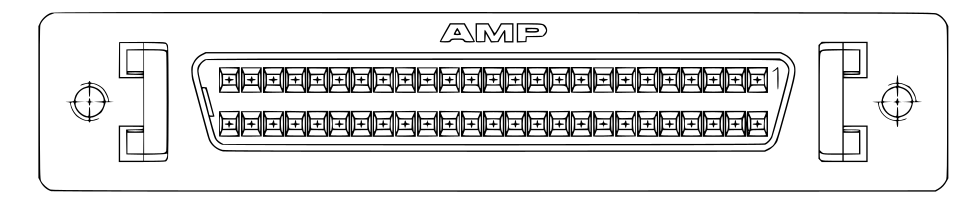
\includegraphics[width=0.6\textwidth]{figures/figure10-scsi2-connector.pdf}
    \caption{External SCSI-2 Connector}
    \label{fig:scsi2connector}
\end{figure}

In the following pinout, a slash (/) preceding the signal name indicates that the signal is active low.

{
\small
\centering
\begin{longtable}{cl|cl}
\toprule
\textbf{Pin} & \textbf{Signal Name} & \textbf{Pin} & \textbf{Signal Name} \\ \midrule
\endfirsthead
\toprule
\textbf{Pin} & \textbf{Signal Name} & \textbf{Pin} & \textbf{Signal Name} \\ \midrule
\endhead

1 & Ground & 26 & /DB(0) \\
2 & Ground & 27 & /DB(1) \\
3 & Ground & 28 & /DB(2) \\
4 & Ground & 29 & /DB(3) \\
5 & Ground & 30 & /DB(4) \\
6 & Ground & 31 & /DB(5) \\
7 & Ground & 32 & /DB(6) \\
8 & Ground & 33 & /DB(7) \\
9 & Ground & 34 & /DB(P) \\
10 & Ground & 35 & Ground \\
11 & Ground & 36 & Ground \\
12 & Reserved & 37 & Reserved \\
13 & Open & 38 & TERMPWR \\
14 & Reserved & 39 & Reserved \\
15 & Ground & 40 & Ground \\
16 & Ground & 41 & /ATN \\
17 & Ground & 42 & Ground \\
18 & Ground & 43 & /BSY \\
19 & Ground & 44 & /ACK \\
20 & Ground & 45 & /RST \\
21 & Ground & 46 & /MSG \\
22 & Ground & 47 & /SEL \\
23 & Ground & 48 & /C/D \\
24 & Ground & 49 & /REQ \\
25 & Ground & 50 & /I/O \\
\bottomrule
\end{longtable}
}

% =============================================================================
% CHAPTER 8: THE A4092 BOOT DISK
% =============================================================================
\chapter{The A4092 Boot Disk}
\label{ch:boot-disk}

The A4092 comes with a boot disk containing utilities and the device driver. When you boot from this disk, you will see the main screen shown in Figure~\ref{fig:bootdisk}.

\begin{figure}[ht]
    \centering
    \includegraphics[width=0.8\textwidth]{figures/amigaos-bootdisk.png}
    \caption{A4092 Boot Disk Main Screen}
    \label{fig:bootdisk}
\end{figure}

The boot disk includes the following utilities:

\begin{itemize}
    \item \textbf{ncr7xx} --- The factory test utility for A4091/A4092 controllers.
    \item \textbf{devtest} --- The best disk benchmarking utility for the Amiga.
    \item \textbf{rdb/RDBFlags} --- Utilities to modify the Rigid Disk Block of your disk. Handle with care.
    \item \textbf{a4092flash} --- The flash update utility for the A4092.
    \item \textbf{update} --- Shortcut to update the A4092 firmware.
    \item \textbf{scsifix} --- Redirects \texttt{scsi.device} accesses to \texttt{a4092.device} for convenience.
\end{itemize}

\section{Updating the Firmware}
\label{sec:updating-firmware}

The A4092 driver firmware can be updated directly from the boot disk. To update the firmware, run the \texttt{Update} program from the boot disk. This will display the update utility shown in Figure~\ref{fig:bootdisk-update}.

\begin{figure}[ht]
    \centering
    \includegraphics[width=0.8\textwidth]{figures/amigaos-bootdisk-update.png}
    \caption{A4092 Firmware Update Utility}
    \label{fig:bootdisk-update}
\end{figure}

Follow the on-screen instructions to complete the firmware update. It is recommended to keep your A4092 firmware up to date to benefit from bug fixes and improvements.

\section{Command Line Firmware Operations}
\label{sec:cli-firmware-operations}

For advanced users, the \texttt{a4092flash} utility provides command-line access to firmware operations:

\begin{itemize}
    \item \texttt{a4092flash -P} --- Check the currently installed firmware version.
    \item \texttt{a4092flash -R backup.rom} --- Backup the current firmware to a file.
    \item \texttt{a4092flash -W a4092.rom} --- Write a new firmware image to the flash.
\end{itemize}

\newpage
\section{Filesystem Support}
\label{sec:filesystem-support}

The A4092 ROM includes CDVDFS, enabling booting from CD-ROM devices. This allows you to boot directly from AmigaOS installation CDs or other bootable media.

Support for FAT16/FAT32 filesystems is also available through the \texttt{fat95} filesystem, which enables reading PC-formatted drives and Zip disks. Adding FAT support requires building and flashing a custom firmware image---refer to the software repository documentation for instructions.

% =============================================================================
% CHAPTER 9: OPTIONAL ACCESSORIES
% =============================================================================
\chapter{Optional Accessories}
\label{ch:optional-accessories}

The A4092 can be enhanced with optional accessories that are available separately from the community. This list is not comprehensive; there are many other community projects worth exploring.

\section{ZuluSCSI}
\label{sec:zuluscsi}

ZuluSCSI is a SCSI device emulator that allows you to use SD cards or other modern storage media in place of traditional SCSI hard drives. The ZuluSCSI firmware and some hardware implementations are open source, though not all hardware implementations are. It connects to the A4092's internal SCSI ribbon cable just like any other SCSI device.

\section{SCSI Knife}
\label{sec:scsi-knife}

\begin{figure}[H]
    \centering
    \includegraphics[width=0.6\textwidth]{figures/figure11-scsiknife.png}
    \caption{SCSI Knife}
    \label{fig:scsiknife}
\end{figure}

The SCSI Knife is a compact ZuluSCSI-based device in a small form factor, designed to fit in tight spaces. It provides the same SCSI emulation capabilities as the full-size ZuluSCSI.

\section{A4092 SCSI Knife Mounting Adapter}
\label{sec:scsi-knife-mounting-adapter}

An optional mounting adapter is available that allows you to attach a SCSI Knife directly to the A4092 board. This provides a clean, integrated solution for adding solid-state SCSI storage to your system without taking up drive bay space.

The mounting adapter connects to the A4092's internal SCSI connector and positions the SCSI Knife securely on the board. Design files are available at \url{https://github.com/A4091/A4092/tree/main/Kicad/Flipper}.

% =============================================================================
% BACK COVER
% =============================================================================
% Add blank page if needed to ensure even page count
\ifodd\value{page}
    \newpage
    \thispagestyle{fancy}
    \fancyhf{}
    \fancyhead[LE,RO]{\textbf{A4092 User's Guide}}
    \fancyfoot[C]{\thepage}
    \null
\fi

% Inside back cover (white, empty)
\newpage
\thispagestyle{empty}
\null

% Back cover (black)
\newpage
\newpagecolor{boxblack}
\thispagestyle{empty}
\null

\end{document}
